\documentclass[aspectratio=43]{beamer}
% \documentclass[aspectratio=169]{beamer}

% Title --------------------------------------------
\title{\Large Street names and Transitional Justice policies}
\author{Francisco Villamil}
\date{STNAMES LAB Workshop\\May 19, 2023}

%%% NOTE -- CHECK THIS: https://github.com/paulgp/beamer-tips


%%% Building heavily on https://github.com/kylebutts/templates

% xcolor, define them
\usepackage{xcolor}

% TEXT COLORS
\definecolor{red}{HTML}{9a2515}
\definecolor{yellow}{HTML}{EBC944}
\definecolor{asher}{HTML}{555F61}
\definecolor{jet}{HTML}{131516}

% THEME COLORS
\definecolor{accent}{HTML}{107895}
\definecolor{accent2}{HTML}{9a2515}

% Color commands
\newcommand\red[1]{{\color{red}#1}}
\newcommand\yellow[1]{{\color{yellow}#1}}
\newcommand\asher[1]{{\color{asher}#1}}

\newcommand\BGred[1]{{\colorbox{red!80!white}{#1}}}
\newcommand\BGyellow[1]{{\colorbox{yellow!80!white}{#1}}}
\newcommand\BGasher[1]{{\colorbox{asher!80!white}{#1}}}


% Beamer Options -------------------------------------

% Background
\setbeamercolor{background canvas}{bg = white}

% Change text margins
\setbeamersize{text margin left = 25pt, text margin right = 15pt}

% \alert
\setbeamercolor{alerted text}{fg = accent2}

% Frame title
\setbeamercolor{frametitle}{bg = white, fg = jet}
\setbeamercolor{framesubtitle}{bg = white, fg = accent}
\setbeamerfont{framesubtitle}{size = \small, shape = \itshape}

% Block
\setbeamercolor{block title}{fg = white, bg = accent2}
\setbeamercolor{block body}{fg = jet, bg = jet!10!white}

% Title page
\setbeamercolor{title}{fg = jet}
\setbeamercolor{subtitle}{fg = accent}

%% Custom \maketitle and \titlepage
\setbeamertemplate{title page}
{
    \begin{centering}
        % \vspace{20mm}
        {\Large \usebeamerfont{title}\usebeamercolor[fg]{title}\inserttitle}\\ \vskip0.25em%
        \ifx\insertsubtitle\@empty%
        \else%
          {\usebeamerfont{subtitle}\usebeamercolor[fg]{subtitle}\insertsubtitle\par}%
        \fi%
        {\vspace{10mm}\insertauthor}\\
        {\color{asher}\small{\insertdate}}\\
    \end{centering}
}

% Table of Contents
\setbeamercolor{section in toc}{fg = accent!70!jet}
\setbeamercolor{subsection in toc}{fg = jet}

% Button
\setbeamercolor{button}{bg = accent}

% Remove navigation symbols
\setbeamertemplate{navigation symbols}{}

% Table and Figure captions
\setbeamercolor{caption}{fg=jet!70!white}
\setbeamercolor{caption name}{fg=jet}
\setbeamerfont{caption name}{shape = \itshape}

% Put slide number / total slides at the bottom right
\makeatother
\setbeamertemplate{footline} %{\hfill\insertframenumber/\inserttotalframenumber}
{%
  \leavevmode%
  \hbox{
  \begin{beamercolorbox}[wd=\paperwidth,ht=2.5ex,dp=1.125ex,leftskip=.3cm,rightskip=.3cm plus1fil]{footlinecolor}%
    \hfill\insertframenumber/\inserttotalframenumber
  \end{beamercolorbox}}%
  \vskip0pt%
}
\makeatletter

% Bullet points

%% Fix left-margins
\settowidth{\leftmargini}{\usebeamertemplate{itemize item}}
\addtolength{\leftmargini}{\labelsep}

%% enumerate item color
\setbeamercolor{enumerate item}{fg = accent}
\setbeamerfont{enumerate item}{size = \small}
\setbeamertemplate{enumerate item}{\insertenumlabel.}

%% itemize
\setbeamercolor{itemize item}{fg = accent!70!white}
\setbeamerfont{itemize item}{size = \small}
\setbeamertemplate{itemize item}[circle]
\setlength{\itemsep}{0pt plus 6pt}

%% right arrow for subitems
\setbeamercolor{itemize subitem}{fg = accent!60!white}
\setbeamerfont{itemize subitem}{size = \small}
\setbeamertemplate{itemize subitem}{$\rightarrow$}

\setbeamertemplate{itemize subsubitem}[square]
\setbeamercolor{itemize subsubitem}{fg = jet}
\setbeamerfont{itemize subsubitem}{size = \small}

% References

%% Bibliography Font, roughly matching aea
\setbeamerfont{bibliography item}{size = \footnotesize}
\setbeamerfont{bibliography entry author}{size = \footnotesize, series = \bfseries}
\setbeamerfont{bibliography entry title}{size = \footnotesize}
\setbeamerfont{bibliography entry location}{size = \footnotesize, shape = \itshape}
\setbeamerfont{bibliography entry note}{size = \footnotesize}

\setbeamercolor{bibliography item}{fg = jet}
\setbeamercolor{bibliography entry author}{fg = accent!60!jet}
\setbeamercolor{bibliography entry title}{fg = jet}
\setbeamercolor{bibliography entry location}{fg = jet}
\setbeamercolor{bibliography entry note}{fg = jet}

%% Remove bibliography symbol in slides
\setbeamertemplate{bibliography item}{}





% Links ----------------------------------------------

\usepackage{hyperref}
\hypersetup{
  colorlinks = true,
  linkcolor = accent2,
  filecolor = accent2,
  urlcolor = accent2,
  citecolor = accent2,
}


% Line spacing --------------------------------------
\usepackage{setspace}
\setstretch{1.2}


% \begin{columns} -----------------------------------
\usepackage{multicol}


% % Fonts ---------------------------------------------
% % Beamer Option to use custom fonts
% \usefonttheme{professionalfonts}
%
% % \usepackage[utopia, smallerops, varg]{newtxmath}
% % \usepackage{utopia}
% \usepackage[sfdefault,light]{roboto}
%
% % Small adjustments to text kerning
% \usepackage{microtype}



% Remove annoying over-full box warnings -----------
\vfuzz2pt
\hfuzz2pt


% Table of Contents with Sections
\setbeamerfont{myTOC}{series=\bfseries, size=\Large}
\AtBeginSection[]{
        \frame{
            \frametitle{Roadmap}
            \tableofcontents[current]
        }
    }


% References ----------------------------------------
\usepackage[
    citestyle= authoryear,
    style = authoryear,
    natbib = true,
    backend = biber
]{biblatex}

% Smaller font-size for references
\renewcommand*{\bibfont}{\small}

% Remove "In:"
\renewbibmacro{in:}{}

% Color citations for slides
\newenvironment{citecolor}
    {\footnotesize\begin{color}{accent2}}
    {\end{color}}

\newcommand{\citetcolor}[1]{{\footnotesize\textcolor{asher}{\citet{#1}}}}
\newcommand{\citepcolor}[1]{{\footnotesize\textcolor{asher}{\citep{#1}}}}

% Tables -------------------------------------------
% Tables too big
% \begin{adjustbox}{width = 1.2\textwidth, center}
\usepackage{adjustbox}
\usepackage{array}
\usepackage{threeparttable, booktabs, adjustbox}

% Fix \input with tables
% \input fails when \\ is at end of external .tex file

\makeatletter
\let\input\@@input
\makeatother

% Tables too narrow
% \begin{tabularx}{\linewidth}{cols}
% col-types: X - center, L - left, R -right
% Relative scale: >{\hsize=.8\hsize}X/L/R
\usepackage{tabularx}
\newcolumntype{L}{>{\raggedright\arraybackslash}X}
\newcolumntype{R}{>{\raggedleft\arraybackslash}X}
\newcolumntype{C}{>{\centering\arraybackslash}X}

% Figures

% \imageframe{img_name} -----------------------------
% from https://github.com/mattjetwell/cousteau
\newcommand{\imageframe}[1]{%
    \begin{frame}[plain]
        \begin{tikzpicture}[remember picture, overlay]
            \node[at = (current page.center), xshift = 0cm] (cover) {%
                \includegraphics[keepaspectratio, width=\paperwidth, height=\paperheight]{#1}
            };
        \end{tikzpicture}
    \end{frame}%
}

% subfigures
\usepackage{subfigure}


% Highlight slide -----------------------------------
% \begin{transitionframe} Text \end{transitionframe}
% from paulgp's beamer tips
\newenvironment{transitionframe}{
    \setbeamercolor{background canvas}{bg=accent!60!black}
    \begin{frame}\color{accent!10!white}\LARGE\centering
}{
    \end{frame}
}


% Table Highlighting --------------------------------
% Create top-left and bottom-right markets in tabular cells with a unique matching id and these commands will outline those cells
\usepackage[beamer,customcolors]{hf-tikz}
\usetikzlibrary{calc}
\usetikzlibrary{fit,shapes.misc}

% To set the hypothesis highlighting boxes red.
\newcommand\marktopleft[1]{%
    \tikz[overlay,remember picture]
        \node (marker-#1-a) at (0,1.5ex) {};%
}
\newcommand\markbottomright[1]{%
    \tikz[overlay,remember picture]
        \node (marker-#1-b) at (0,0) {};%
    \tikz[accent!80!jet, ultra thick, overlay, remember picture, inner sep=4pt]
        \node[draw, rectangle, fit=(marker-#1-a.center) (marker-#1-b.center)] {};%
}


\begin{document}
% ====================================================

% ----------------------------------------------------
\begin{frame}
  \titlepage
\end{frame}
% ----------------------------------------------------

% ----------------------------------------------------
\begin{frame}
\frametitle{Street names and TJ}
\centering

\begin{itemize}
  \item<1-> What is Transitional Justice?
  \begin{itemize}
    \item Set of policies implemented during transitions, usually from authoritarianism or conflict, with various goals (normative and positive)
    \item Prosecutions, truth commissions, reparations, \textbf{symbolic policies}
  \end{itemize}
  \item<2-> Symbolic TJ policies usually aimed at public displays of the past and mechanisms of ``prestige allocation''
  \item<2-> Public monuments, memorials, museums, street names, etc
  \item<3-> Related to idea of toponymy as cultural markers, but probably more contested $\rightarrow$ research question
\end{itemize}

\end{frame}
% ----------------------------------------------------

% ----------------------------------------------------
\begin{frame}
\frametitle{Street names and TJ}
\centering

\begin{itemize}[<+->]
  \item Focusing on change of symbols after transitions, i.e. street names
  \item Street names removal implies changing public spaces, who gets recognition in them, societal role models, etc
  \item This means that both the \textit{causes} \& \textit{consequences} of those changes are relevant, opening up different related questions, e.g.
  \begin{itemize}
    \item political motivations behind the changes
    \item long-term effects on attitudes
    \item short-term political reaction (e.g. backlash?), etc
  \end{itemize}
  \item Today, focus on \textbf{short-term political (electoral) consequences}
\end{itemize}

\end{frame}
% ----------------------------------------------------

% ----------------------------------------------------
\imageframe{img/rap_paper}
% ----------------------------------------------------

% ----------------------------------------------------
\begin{frame}
\frametitle{Spanish context}
\centering

\begin{itemize}
  \item<1-> Civil War (1936--1939) and Francoist regime (1939--1975)
  \item<1-> Transition to democracy after 1977
  \begin{itemize}
    \item Negotiated transition, 1977 Amnesty Law \& `Pact of Forgetting'
  \end{itemize}
  \item<2-> Unequal removal of public symbols linked to Francoism
  \begin{itemize}
    \item Some municipalities unilaterally removed all or some symbols, including street names, in the 1980s
    \item[] {\scriptsize (e.g. Basque Country and Catalonia removed virtually all street names; in Madrid, Av. del Generalísimo became P. de la Castellana in 1980)}
  \end{itemize}
  \item<2-> Many symbols remained, from statues of Franco to street names
  \item<3-> Social and political change around 2000
  \begin{itemize}
    \item New social movements, renewed demand for revision of the past, etc
    \item Domestic (grandchildren) and international (rise of TJ) factors
  \end{itemize}
\end{itemize}

\end{frame}
% ----------------------------------------------------

% ----------------------------------------------------
\begin{frame}
\frametitle{2007 Law of Historical Memory}
\centering

\begin{itemize}
  \item<1-> TJ law mainly focused on truth-seeking and symbolic measures
  \item<1-> Compulsory removal of Francoist symbols from public spaces, including \textbf{street names}
  \item<2-> LHM was weakly enforced: many municipalities did change street names, but many remained
  \item<2-> National dynamics: 2008 economic crisis, right-wing government after 2011 (and similar shift in local councils)
\end{itemize}

\end{frame}
% ----------------------------------------------------

% ----------------------------------------------------
\begin{frame}
\frametitle{Francoist streets by year}
\centering

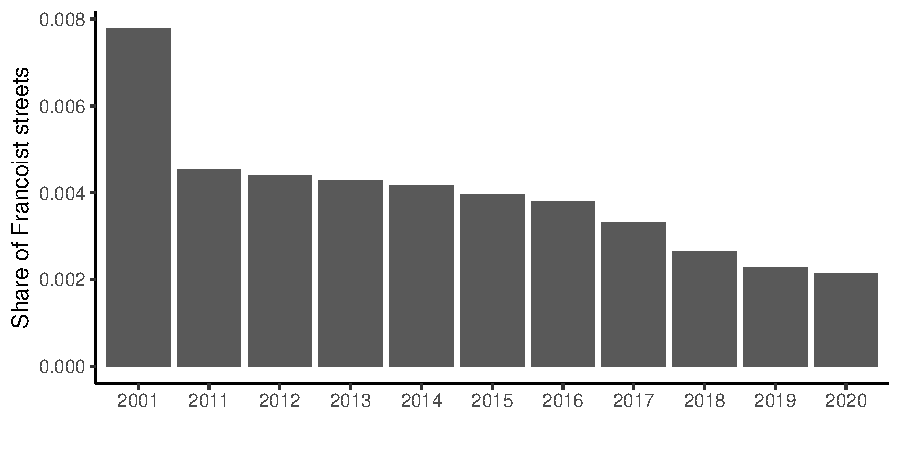
\includegraphics[width = \textwidth]{../descriptives/output/fs_by_year}

\end{frame}
% ----------------------------------------------------

% ----------------------------------------------------
\begin{frame}
\frametitle{2007 Law of Historical Memory}
\centering

\begin{itemize}[<+->]
  \item Even if local govts did not implement the LHM, it was still illegal to keep Francoist names
  \item Civic associations started to sue
  \item Things started to change after 2015
  \begin{itemize}
    \item Legal battles
    \item Electoral cycle
  \end{itemize}
\end{itemize}

\end{frame}
% ----------------------------------------------------

% ----------------------------------------------------
\imageframe{img/olmedo}
% ----------------------------------------------------

% ----------------------------------------------------
\imageframe{img/madrid_carmena}
% ----------------------------------------------------

% ----------------------------------------------------
\imageframe{img/principado}
% ----------------------------------------------------

% ----------------------------------------------------
\begin{frame}
\frametitle{Francoist street removals over time}
\centering

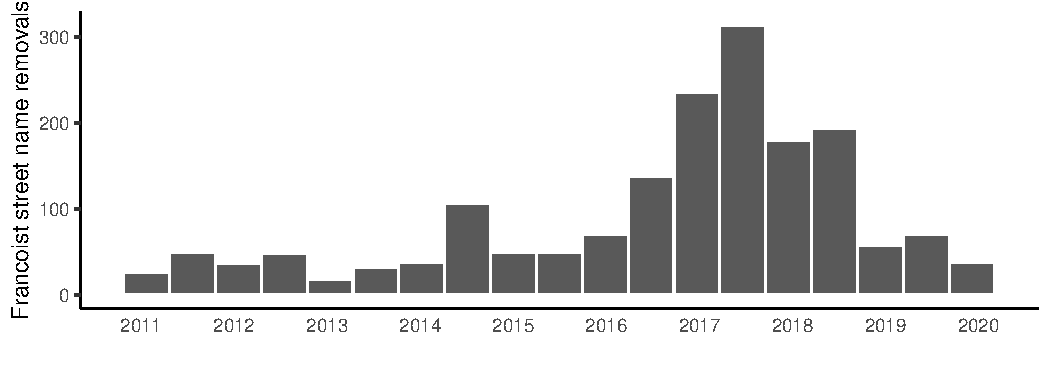
\includegraphics[width = \textwidth]{../descriptives/output/changes_by_year}

\end{frame}
% ----------------------------------------------------

% ----------------------------------------------------
\begin{frame}
\frametitle{RQ and design basics}
\centering

\begin{itemize}[<+->]
  \item What are the consequences of removing street names?
  \item Looking at local-level effects on electoral behaviour, particularly vote for the far-right party Vox
  \item Using a Diff-in-Diff design between 2016 and 2019 elections
  \item Compare municipalities that removed Francoist streets during 2016--19 to those that did not, \textit{only} among those that still had them in June 2016
  \begin{itemize}
    \item Key ID assumption: changes during this period were relatively exogenous to local electoral dynamics
  \end{itemize}
\end{itemize}

\end{frame}
% ----------------------------------------------------

% ----------------------------------------------------
\imageframe{../descriptives/output/map_full}
% ----------------------------------------------------

% % ----------------------------------------------------
% \imageframe{../descriptives/output/map}
% % ----------------------------------------------------

% ----------------------------------------------------
\begin{frame}
\frametitle{What are we measuring looking at Vox?}
\centering

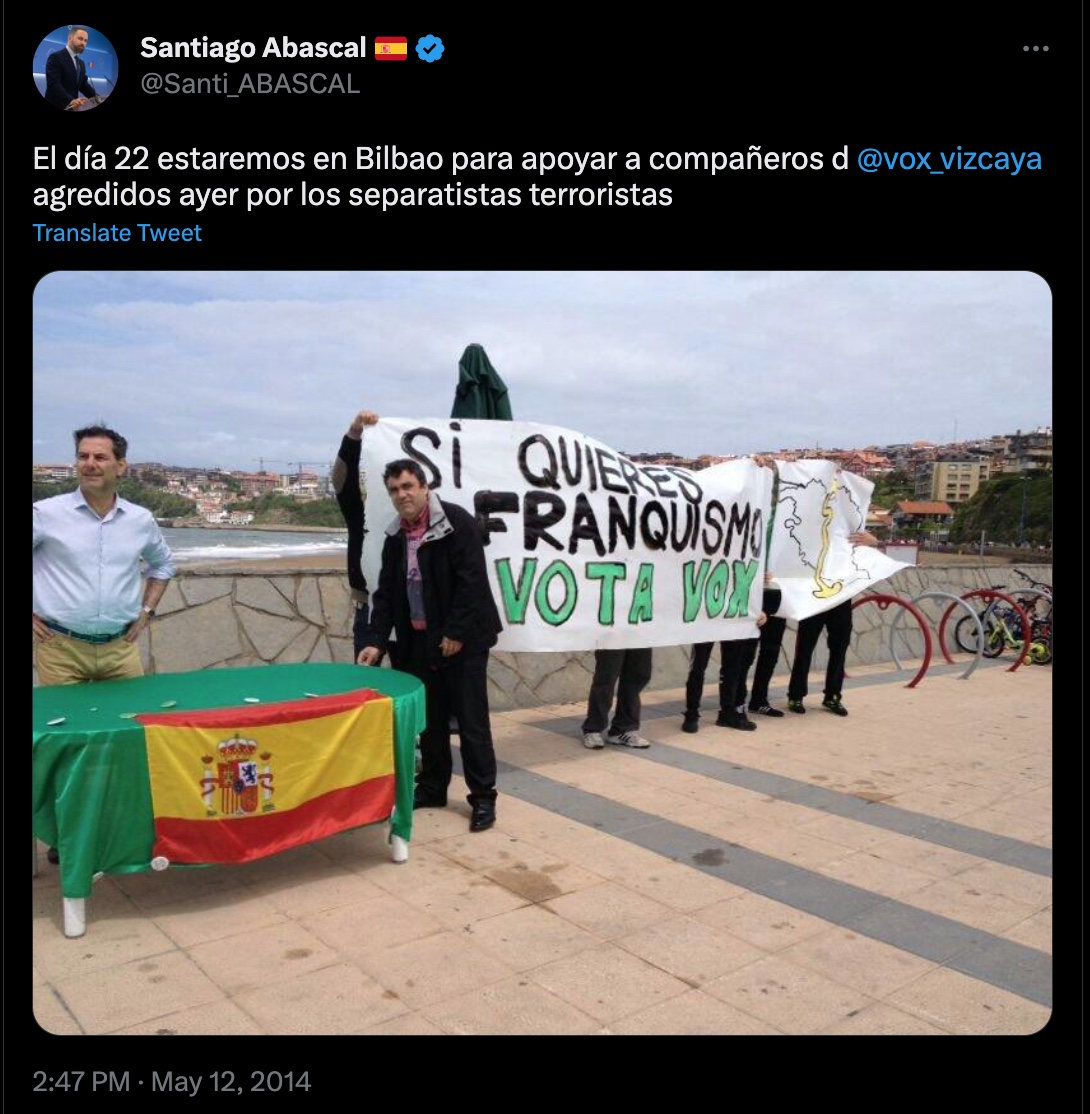
\includegraphics[width = .7\textwidth]{img/vox_franquismo}

\end{frame}
% ----------------------------------------------------

% ----------------------------------------------------
\begin{frame}
\frametitle{Data}
\centering

\begin{itemize}
  \item<1-> \textbf{Outcome}: local share of votes for Vox (and PP \& PSOE)
  \begin{itemize}
    \item June 2016 and April 2019 elections
    \item (We also look at prior trends, esp. for PP/PSOE)
  \end{itemize}
  \item<2-> \textbf{Independent variable}: Francoist street name removal between June 30, 2016 and December 31, 2018
  \begin{itemize}
    \item Coding changes from INE \textit{callejero} data
    \item Coded Francoist streets from Madrid commission list + additions
  \end{itemize}
  \item<3-> \textbf{Controls}: turnout (2016), population (2011), number of Francoists streets, unemployment rate, leftist mayor in 2015, region FE
\end{itemize}

\end{frame}
% ----------------------------------------------------

% ----------------------------------------------------
\begin{frame}
\frametitle{Results}
\centering

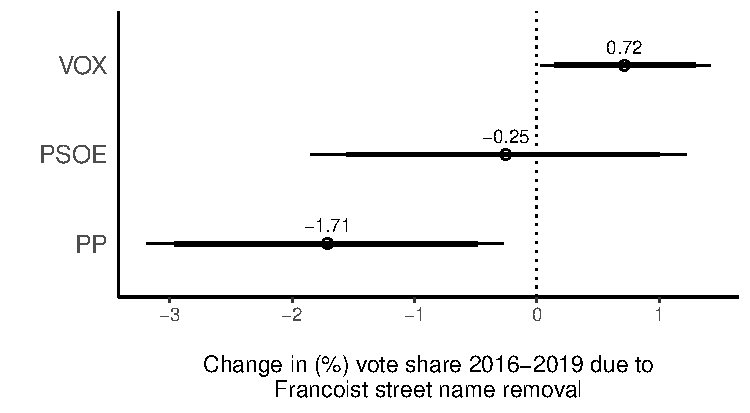
\includegraphics[width = \textwidth]{../main_models/output/DiD_estimates}

\end{frame}
% ----------------------------------------------------

% ----------------------------------------------------
\imageframe{../descriptives/output/par_trends_norm}
% ----------------------------------------------------

% ----------------------------------------------------
\begin{frame}
\frametitle{Conclusion}
\centering

\begin{itemize}[<+->]
  \item Evidence for backlash over symbolic TJ
  \item But maybe too soon to say TJ is bad, as some argue:
  \item[1.] These are short-term effects, what happens in the long term?
  \item[2.] Should we blame the street name removal or the parties that take advantage of it?
  \item[3.] No need to throw the baby out with the bathwater
  \begin{itemize}
    \item Explore combination of TJ measures, complement symbolic TJ with other policies (education, `marketing', etc)
  \end{itemize}
\end{itemize}

\end{frame}
% ----------------------------------------------------

% ----------------------------------------------------
\begin{frame}
\frametitle{Future research with streets data}
\centering

\begin{itemize}
  \item<1-> What issues generate a backlash over public recognition?
  \begin{itemize}
    \item e.g. would we see a similar pattern of backlash against `woke ideologies' if streets were renamed to achieve gender balance?
  \end{itemize}
  \item<2-> Problems of identification
  \begin{itemize}
    \item Could we analyze effects in the long term?
    \item In a way, this is a LATE, how to generalize to the whole country?
    \item What is the correct unit of analysis? (perhaps smaller, larger?)
  \end{itemize}
  \item<3-> Beyond Spain and streets
  \begin{itemize}
    \item Other types of toponymy? (less variation)
    \item Processes in other countries, what account for renaming?
  \end{itemize}
\end{itemize}

\end{frame}
% ----------------------------------------------------

% ----------------------------------------------------
\begin{frame}
\frametitle{}
\centering

Thank you!

\end{frame}
% ----------------------------------------------------

% ----------------------------------------------------
\begin{frame}
\frametitle{}
\centering

-- Extra slides --

\end{frame}
% ----------------------------------------------------

% ----------------------------------------------------
\begin{frame}
\frametitle{Francoist street names}
\centering

\setstretch{0.8}
{\tiny 18 de Julio; Alcalde Conde de Mayalde; Alcazar; Alcazar de Toledo; Alferez Provisional; Almirante Francisco Moreno; Angel del Alcazar; Arco de la Victoria; Arriba Espana; Aunos; Batalla de Belchite; Batalla del Ebro; Caidos; Caidos (de Los); Caidos (los); Caidos de la Division Azul; Caidos Por la Patria; Calvo Sotelo; Calvo Sotelo (de); Capita Cortes; Capitan Cortes; Capitan Cortes (del); Capitan Haya; Capitan Luna; Carlos Pinilla; Carlos Ruiz; Carrero Blanco; Caudillo; Caudillo (del); Cerro de Garabitas; Cirilo Martin Martin; Comandante Franco; Comandante Franco; Comandante Zorita; Conde Vallellano; Crucero Baleares; Defensores del Alcazar; Defensores del Alcazar; Dieciocho de Julio; Diego Salas Pombo; Division Azul; Doctor Vallejo-Nagera; Eduardo Aunos; Ejercito Espanol; El Algabeno; Emilio Jimenez Millas; Falange Espanola; Federico Mayo; Federico Servet; Fernandez Ladreda; Francisco Franco; Franco; Garcia Morato; General; General Aranda; General Asensio Cabanillas; General Cabanellas; General Cabanellas; General Davila; General Fanjul; General Franco; General Garcia de la Herranz; General Garcia Escamez; General Kirkpatrick; General Millan Astray; General Mola; General Mola (del); General Moscardo; General Munoz Grandes; General Orgaz; General Primo de Rivera; General Queipo de Llano; General Rodrigo; General Romero Basart; General Sagardia Ramos; General Saliquet; General Sanjurjo; General Varela; General Yague; Generalisimo; Generalisimo (del); Generalisimo Franco; Gobernador Carlos Ruiz; Hermanos Falco y Alvarez de Toledo; Hermanos Garcia Noblejas; Heroes del Alcazar; Jose Antonio; Jose Antonio (de); Jose Antonio Giron; Jose Antonio Giron; Jose Antonio Primo de Rivera; Jose Luis de Arrese; Jose Maria Peman; Juan Pujol; Juan Vigon; Lepanto; Los Martires; Manuel Sarrion; Martires; Martires (los); Matias Montero; Millan Astray; Munoz Grandes; Onesimo Redondo; Pilar Primo de Rivera; Primero de Octubre; Primo de Rivera; Puerto de los Leones; Queipo de Llano; Ramiro Ledesma; Ramon Franco; Ruiz de Alda; Salas Pombo; Veintiocho de Marzo}\\

\end{frame}
% ----------------------------------------------------

% ----------------------------------------------------
\begin{frame}
\frametitle{Sample descriptives}
\centering

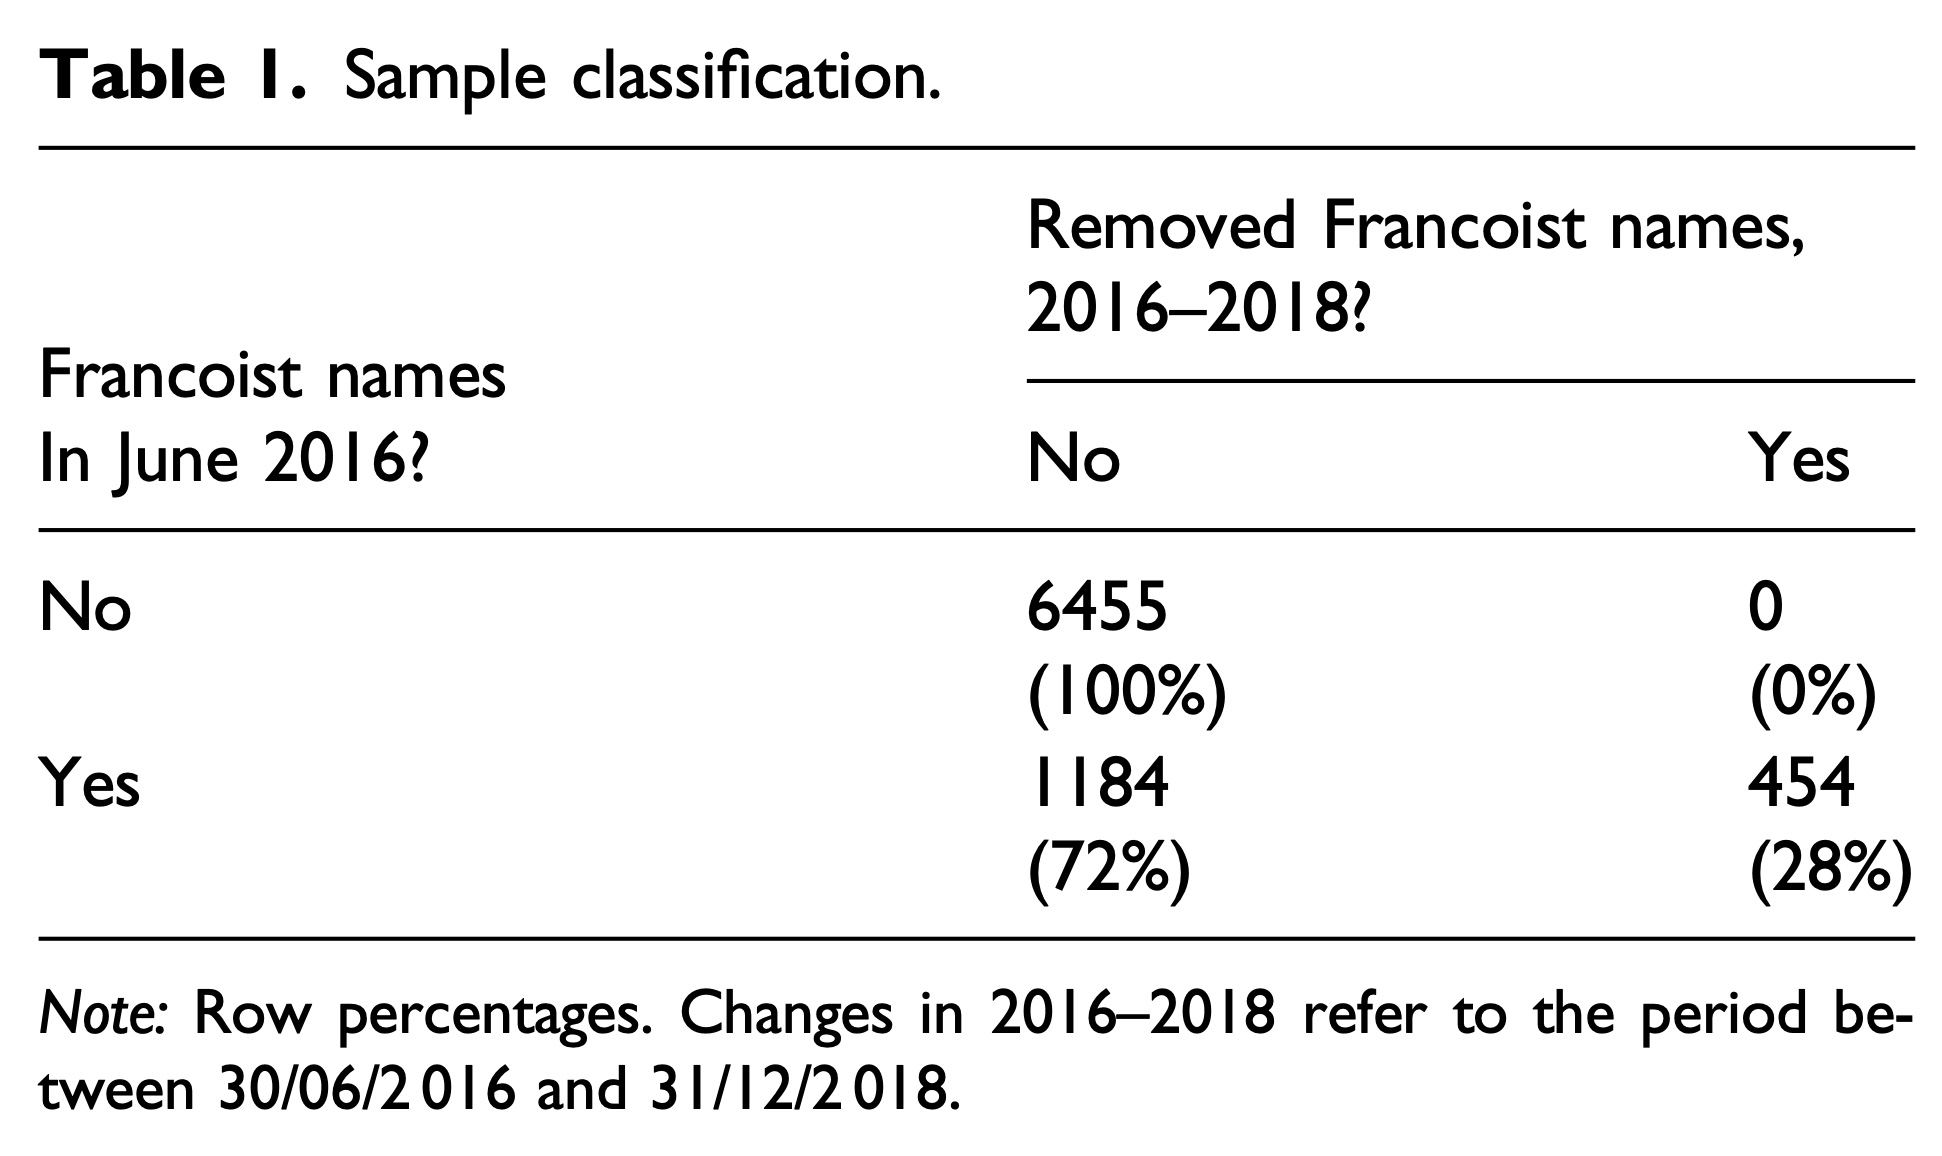
\includegraphics[width = \textwidth]{img/table_sample}

\end{frame}
% ----------------------------------------------------

% ----------------------------------------------------
\imageframe{../descriptives/output/changes_by_prov}
% ----------------------------------------------------

% ----------------------------------------------------
\imageframe{../descriptives/output/trt_strength_st2016}
% ----------------------------------------------------

% ----------------------------------------------------
\begin{frame}
\frametitle{Street names and TJ}
\centering

\begin{itemize}
  \item Difference with other non-transitional changes? (e.g. gender)
  \begin{itemize}
    \item Periods of political violence usually more divisive, deeper link with social and political cleavages
    \item Potentially, different dynamics: more concentrated in time and linked or enforced to nation-level legal framework
    \item But whether and how much it applies is an open question
  \end{itemize}
\end{itemize}

\end{frame}
% ----------------------------------------------------

% ====================================================
\end{document}
